\subsection{Planung}\label{cap:methoden_planung}


\begin{figure}[ht]
    \begin{center}
      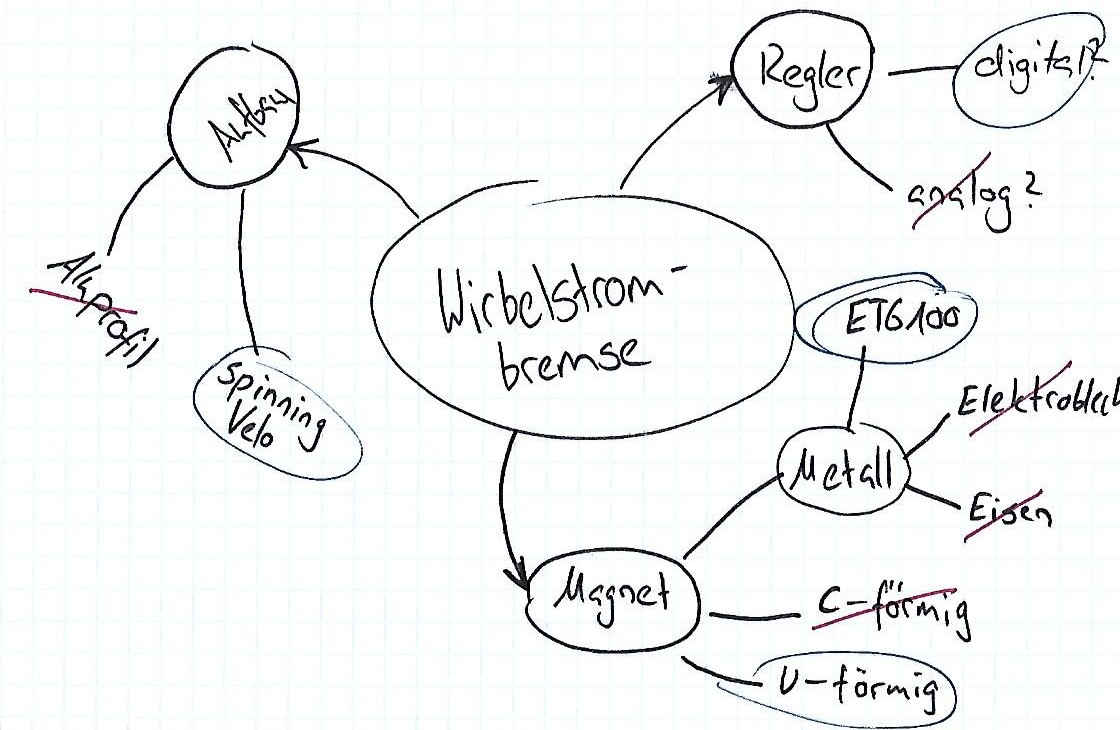
\includegraphics[width=12cm]{assets/images/planung}
    \end{center}
    \vspace{-3ex}
    \caption{Mindmap}
    \label{fig:mindmap}
  \end{figure}
Der erste Schritt zum Erreichen der Hypothese war die Ausarbeitung der Vorgehens-Struktur. Bevor mit dem Aufbau der Struktur begonnen werden konnte, kam es zu Unklarheiten. Insbesondere wie genau die Hypothese erreicht werden konnte, da noch kein Plan existierte, weder wie der Aufbau der Wirbelstrombremse noch wie die Regelung erstellt werden sollte. Diese Unklarheiten konnten durch eine Ideenfindung geklärt werden. Wurden genügend Ideen gesammelt, konnten diese in eine Vorgehens-Struktur eingesetzt werden, wobei das Ziel die Erreichung der Hypothese darstellte.
\newpara
Nachdem eine Ideenfindungen stattgefunden hatte, konnte ein Vorgehen aufgebaut werden. Jeder Vorschlag wurde bearbeitet und anhand der Priorität des Vorschlags eine Zeit zugeteilt, welche für die Verarbeitung benötigt wird. Diese Planung ähnelt dem \textit{Scrum}, nur dass keine Sprints und deren zugehörigen Sprint-Reviews geplant wurde.
\newpara
\begin{tcolorbox}
  \textit{Scrum} ist ein Projektmanagementsystem, welches ein Team erlaubt in Sprints Aufträge zu bearbeiten. Diese Aufträge werden in einem Sprint-Review anhand der gesetzten Ziele überprüft und je nach Ergebnis werden nicht erreichte Aufträge im nächsten Sprint weiterverarbeitet (\cite{scrum_info}). 
\end{tcolorbox}
\newpara

\begin{figure}[ht]
    \begin{center}
      \begin{tikzpicture}
        \node[emptynode]     (a1)                                        {$A_1$};
        \node[emptynode]     (a2)   [below= 2cm of a1]                     {$A_2$};
        \node[emptynode]     (z)    [below right= 0.9cm and 5cm of a1]                     {Z};
        \node[emptynode]     (e1)   [right= 2cm of a1]                                  {};
        \node[emptynode]     (e2)   [right= 2cm of a2]                     {};
        \node[emptynode]     (e3)   [below right= 1cm and 3cm of a1]                     {};
  
        \draw [-] (a1) -- (e1.center);
        \draw [-] (a2) -- (e2.center);
        \draw [-] (e2.center) -- (e3.center);
        \draw [-] (e1.center) -- (e3.center);
        \draw [arrow_right] (e3.center) -- (z);
      \end{tikzpicture}
    \end{center}
    \vspace{-3ex}
    \caption{Parallele Vorgehensweise}
    \label{fig:planung_a1a2_bis_z}
  \end{figure}
Zu Beginn wurde eine Art paralleles Vorgehen geplant (Siehe Abbildung \ref{fig:planung_a1a2_bis_z}). Ziel dieses Vorgehens war die Aufteilung des Elektronik-Teils und des Mechanik-Teils. Dies erlaubte die Ausführung zweier Schritte gleichzeitig, was zum schnelleren Arbeiten hätte führen sollen. In anderen Worten wurde mit Schritt $A_1$ und $A_2$, welche den Elektronik-Teil und den Mechanik-Teil repräsentieren, begonnen und vor dem Abschluss bei Schritt $Z$ werden die beiden Schritte verschmelzt.
\newpara
\begin{figure}[ht]
    \begin{center}
      \begin{tikzpicture}
        \node[emptynode]     (a)                                           {A};
        \node[emptynode]     (z)   [right= 5cm of a]                     {Z};

  
        \draw [arrow_right] (a) -- (z);

      \end{tikzpicture}
    \end{center}
    \vspace{-3ex}
    \caption{Einfache Vorgehensweise}
    \label{fig:planung_a_bis_z}
  \end{figure}
Später musste aber dieses Vorgehen verworfen werden, da die Planung des Magneten einige Schwierigkeiten brachte, welche im Kapitel \ref{cap:methoden_magnet_design} erläutert werden. Die neue Struktur basierte auf einer einfachen Vorgehensweise (Siehe Abbildung \ref{fig:planung_a_bis_z}). Es wurde mit Schritt A begonnen und endete schlussendlich mit Schritt Z, welche die Erreichung der Hypothese darstellte.